\documentclass[../thesis-main.tex]{subfiles}

\begin{document}

\chapter{Isch\ae{}mic Variation}
\label{ch:ischaemia}

\begin{aquote}{Source}
  {\fontencoding{T1}\fontfamily{pzc}\selectfont
   Quotation
  }
\end{aquote}
\rule{\linewidth}{0.25mm}

\begin{quote}
 \emph{This chapter presents insights into the isch\ae{}mic parameter space. A brief introduction is given to the work, and the justification behind the methodology used here. The changes of the parameter space defined in the previous chapter are discussed, followed by an analysis of the effects of the isch\ae{}mic parameter space itself. The possible consequences of model failure are discussed.}
\end{quote}

\section{Variation Within Isch\ae{}mia}
\label{sec:ischaemia-rationale}
As has previously been commented upon, computational modelling of variation is promising new insights into the causes and consequences of variation. Coupled to this progress in computational modelling are the benefits when investigating isch\ae{}mia: due to the rapidly changing nature of the isch\ae{}mic milieu, comprehensive experimental validation of hypotheses is difficult. Computational modelling allows a rapid, flexible manner with which to test hypotheses regarding isch\ae{}mia. This is especially useful for assessing the import of factors that are difficult to constrain and control experimentally.

This work presents the first time, to the author's knowledge, where a comprehensive model population approach has been applied to the isch\ae{}mic environment. Furthermore, the parameter space methodology is applied to the isch\ae{}mic environment itself. This provides two important possible benefits. First of all, in the same way that the previous chapter postulated variation in the model itself as being partly responsible for natural variation, it is reasonable to extend this same postulate of variability, and thus the methodology used, to the environment itself. Secondly, it can be remembered that isch\ae{}mia rarely exists in isolation, and that there is commonly a `border zone' that exists between the central isch\ae{}mic zone and the surrounding healthy tissue. As was commented upon in \S\ref{subsubsec:isch-ap}, the changes in environmental conditions associated with isch\ae{}mia do not vary in a spatially uniform manner---Fig.\ref{fig:spatial-ischaemia} in that section (originally from \citet{Tice2007}) demonstrates that it can be expected that hyperkal\ae{}mic conditions can exist while other environmental changes associated with isch\ae{}mia are not present. Performing a parameter space search allows us to examine this spatial variation.

The inclusion of variation in isch\ae{}mia modelling is of potentially key importance. It is already known through significant previous literature (see \S\ref{sec:disease} for a review) that isch\ae{}mia provides an arrhythmogenic substrate. It has also been demonstrated that arrhythmogenesis is favoured in heterogeneic substrate---indeed, \citet{Tice2007} demonstrated that the heterogeneity introduced by changes from the central isch\ae{}mic zone, to the border zone, to normal tissue, can provide the substrate for arrhythmias.

It is based on these observations that the primary hypothesis being tested here is: does the application of isch\ae{}mic conditions lead to an increase in heterogeneity within the population that could, in tissue, be arrhythmogenic? To put it another way, one could ask whether the benign variation that is being modelled by the population then transitions to malign variation under isch\ae{}mic conditons. It should be remembered that the results presented in this work cannot be said to imply arrhythmogenesis, which is a super-cellular behaviour. However, there is a silver lining to the simulation of isch\ae{}mia---since it has been noted that isch\ae{}mia reduces the extent of cell-coupling, it is implied that the results presented here will be ameliorated to a lesser degree by any cell-coupling.

The work presented in this chapter will also examine the importance of studying population responses, and the aspects of these responses that would not be observed using single model simulations.

In this chapter, it must be remembered that the term '$x$ minutes post-occlusion (PO)' is used as short-hand, and it is wise to consider the data presented with such a label in terms of the underlying conditions instead; the corresponding values are given in Table~\ref{table:isch-params}.
\begin{table}
 \centering
 \begin{tabular}{c|cccccc}
  Time (min PO) & 0 & 2 & 4 & 6 & 8 & 10 \\
  \hline
  \hline
  \ko{} (mM) & 5.40 & 7.72 & 10.04 & 12.36 & 14.68 & 17.00 \\
  \fkatp{} ($\%$) & 0.00 & 0.16 & 0.32 & 0.48 & 0.64 & 0.80 \\
  \finhib{} ($\%$) & 0 & 5 & 10 & 15 & 20 & 25 \\
  \fna{} ($\%$) & 0 & 6 & 12 & 18 & 24 & 30
 \end{tabular}
 \caption[Isch\ae{}mic environment parameters]{Table showing what parameters are used in simulation to approximate a given time post-occlusion. \fkatp{} represents the degree of activation of \ikatp{}, \finhib{} represents the degree of inhibition applied to \ina{} and \ica{}, and \fna{} represents the percentage increase/decrease in \nai{} and \inak{}, respectively.}
 \label{table:isch-params}
\end{table}

As a further matter of nomenclature in this chaper, two different measures of variation are used in this chapter: the variance and the range (defined as the difference between the maximum and the minimum values found amongst the population for a given set of environmental conditions. When both measures demonstrate the same trend, the term variation shall be used directly. It must also be considered that it is not always sufficient to use simply these measures, but sometimes to examine the data directly---such measures will be used in the following analysis.

\section{Population Response to Isch\ae{}mia}
\label{sec:isch-population}
The APs for the population at various discrete points during isch\ae{}mia are shown in Fig.~\ref{fig:isch-ap-apd90}, with histograms representing the APD\sub{90} values for the populations also shown. Associated data for the mean, standard deviation and range responses for common biomarkers for both populations are shown in Table~\ref{table:isch-stats}.

Both populations show a qualitative and quantitative (based on mean population response) agreement with expected AP response (increase in \vrest{}, decrease in \dvdtmax{} and APD\sub{90}). However, the AP morphology of the two populations, while initially similar, shows different population-level responses to isch\ae{}mia. The Shannon population demonstrates secondary depolarisation as isc\ae{}mia progresses, \idest{} beyond 4 min PO, \vmax{} is not reached during the initial upstroke, but rather during secondary depolaristion during Phase 2 of the AP. It should be noted that this increased prominence of the dome in the AP is not due to an increase in the dome itself, but rather the decline of the initial upstroke occurs at a far greater rate. The Mahajan population initially shows the same process---the dome phase of the AP is less affected by the progression of isch\ae{}mia, and 6 min PO \vmax{} occurs during Phase 2. However, at 8 min PO some models in the Mahajan population exhibit a phenomenon that shall be termed `dome collapse', \idest{} the dome exhibited during Phase 2 is no longer sustained; this shall be explored in further detail in \S\ref{subsec:isch-apd90-response}. It can be noted that the two populations demonstrate different sensitivities to isch\ae{}mic conditions, and indeed that the population response can go in opposite directions for the same  change; these differences shall be expanded upon for specific biomarkers responses.
\begin{figure}
 \centering
 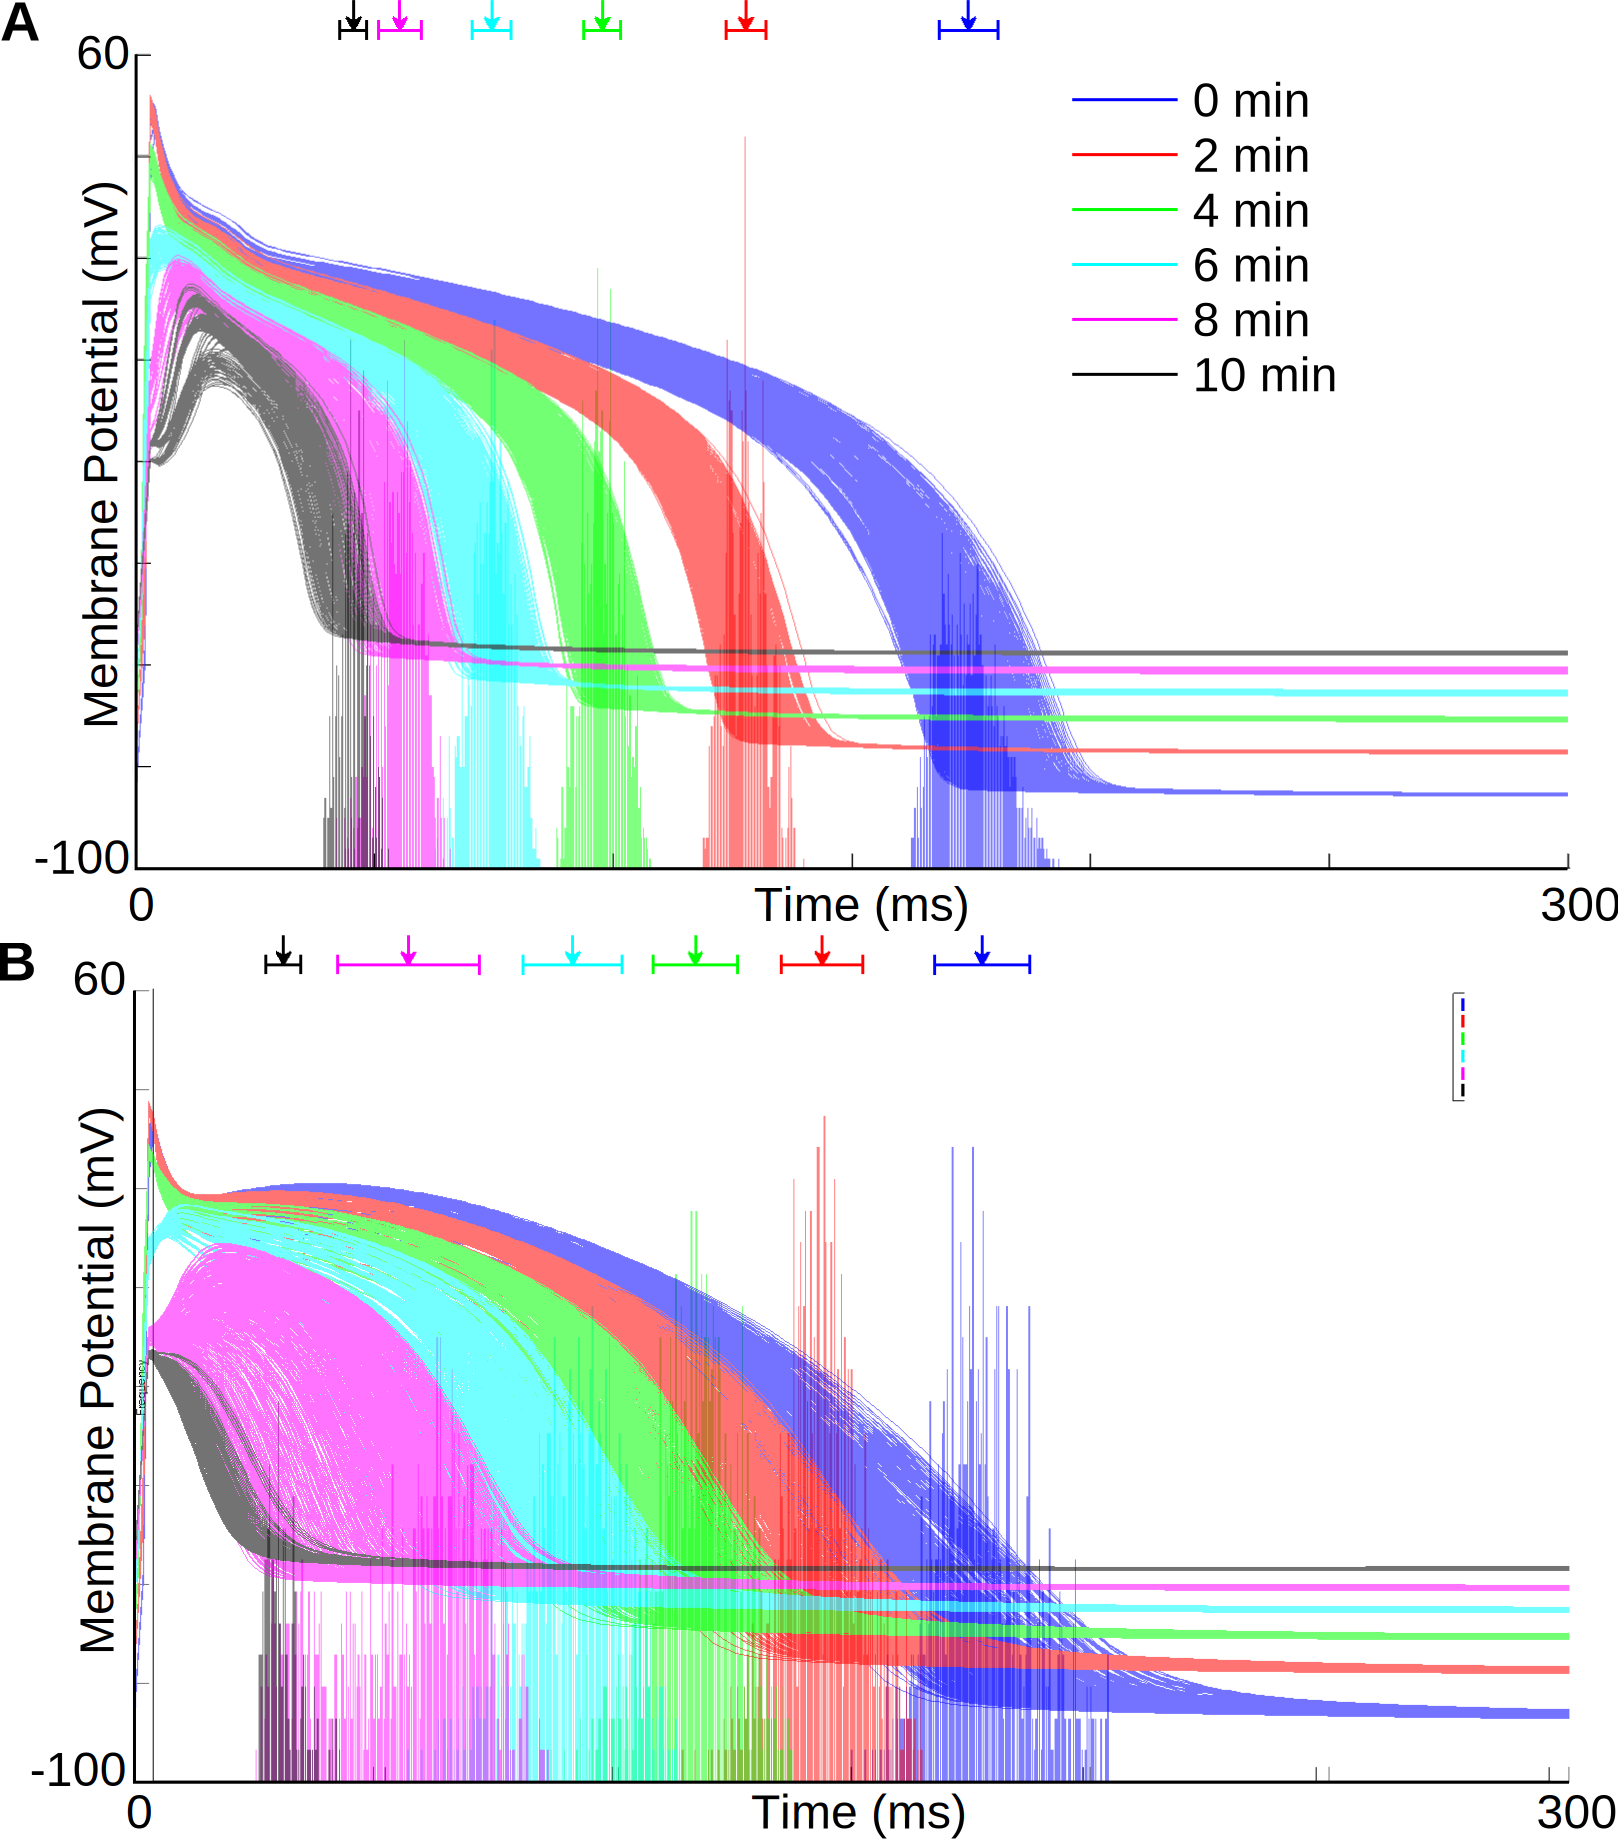
\includegraphics[width=0.8\textwidth]{isch17-ap-apd90}
 \caption[Effect of different degrees of isch\ae{}mia on the Shannon and Mahajan model populations.]{Effect of different degrees of isch\ae{}mia on the Shannon and Mahajan model populations. AP traces for non-failing models of the Shannon and Mahajan populations are shown in (A) and (B), respectively, with histograms of the APD\sub{90} values associated with these traces shown in (C, Shannon) and (D, Mahajan). In (C) and (D), the arrows at the top of the figures indicate the mean APD\sub{90} of the population, with the bars representing plus/minus standard deviation from the mean.}
 \label{fig:isch-ap-apd90}
\end{figure}

% Mahajan more sensitive to ischæmic changes than Shannon

\subsection{APD\sub{90}}
\label{subsec:isch-apd90-response}
For both model populations, progression of isch\ae{}mia works to reduce population variation in its early stages (until 4 min PO)---beyond this point, the response is population-dependent (Fig.~\ref{fig:isch-ap-apd90} and Table~\ref{table:isch-stats}).

% Data for [K+]o(isch) = 17 mM
\begin{table}
 \centering
 \begin{tabular}{ccc|cccccc}
  & & & \multicolumn{6}{c}{Time PO (min)} \\
  & & & 0 & 2 & 4 & 6 & 8 & 10 \\
  \hline
  \hline
  \multirow{9}{*}{Shannon} & \multirow{3}{*}{APD\sub{90}} & Mean & $174.1$ & $127.4$ & $97.4$ & $74.2$ & $55.0$ & $45.3$ \\
  & & Std & $6.23$ & $4.17$ & $3.89$ & $4.14$ & $4.44$ & $2.82$ \\
  & & Range & $30.9$ & $20.9$ & $19.7$ & $21.8$ & $23.5$ & $13.5$ \\
  \cline{2-9}
  & \multirow{3}{*}{ERP} & Mean & $175.9$ & $132.7$ & $107.5$ & $93.2$ & $94.8$ & $182.9$ \\
  & & Std & $6.20$ & $4.21$ & $3.85$ & $3.77$ & $2.87$ & $31.47$ \\
  & & Range & $30.7$ & $21.3$ & $19.5$ & $19.9$ & $15.5$ & $324.0$ \\
  \cline{2-9}
  & \multirow{3}{*}{PRR} & Mean & $1.8$ & $5.3$ & $10.1$ & $19.0$ & $39.8$ & $137.6$ \\
  & & Std & $0.09$ & $0.19$ & $0.23$ & $0.49$ & $1.96$ & $31.94$ \\
  & & Range & $0.4$ & $1.1$ & $1.1$ & $2.1$ & $8.2$ & $319.9$ \\
  \hline
  \multirow{9}{*}{Mahajan} & \multirow{3}{*}{APD\sub{90}} & Mean & $177.9$ & $143.6$ & $116.3$ & $90.0$ & $54.7$ & $27.8$ \\
  & & Std & $10.20$ & $8.77$ & $9.04$ & $10.64$ & $15.25$ & $3.75$ \\
  & & Range & $55.0$ & $51.4$ & $54.0$ & $58.4$ & $62.5$ & $17.4$ \\
  \cline{2-9}
  & \multirow{3}{*}{ERP} & Mean & $174.2$ & $148.7$ & $128.0$ & $112.0$ & $100.8$ & $600.0$ \\
  & & Std & $9.32$ & $8.82$ & $9.43$ & $11.44$ & $18.31$ & $0.00$ \\
  & & Range & $50.2$ & $51.4$ & $56.2$ & $63.3$ & $77.5$ & $0.0$ \\
  \cline{2-9}
  & \multirow{3}{*}{PRR} & Mean & $-3.7$ & $5.1$ & $11.7$ & $22.0$ & $46.1$ & $572.2$ \\
  & & Std & $1.98$ & $0.32$ & $0.48$ & $0.91$ & $3.17$ & $3.75$ \\
  & & Range & $7.9$ & $2.0$ & $2.3$ & $5.0$ & $15.5$ & $17.4$
 \end{tabular}
 \caption[Isch\ae{}mic Effect on Model Populations]{Effect of different degrees of isch\ae{}mic severity on the population level response for common biomarkers for the Mahajan and Shannon frameworks, according to mean, standard deviation (Std) and range.}
 \label{table:isch-stats}
\end{table}

\begin{figure}
 \centering
 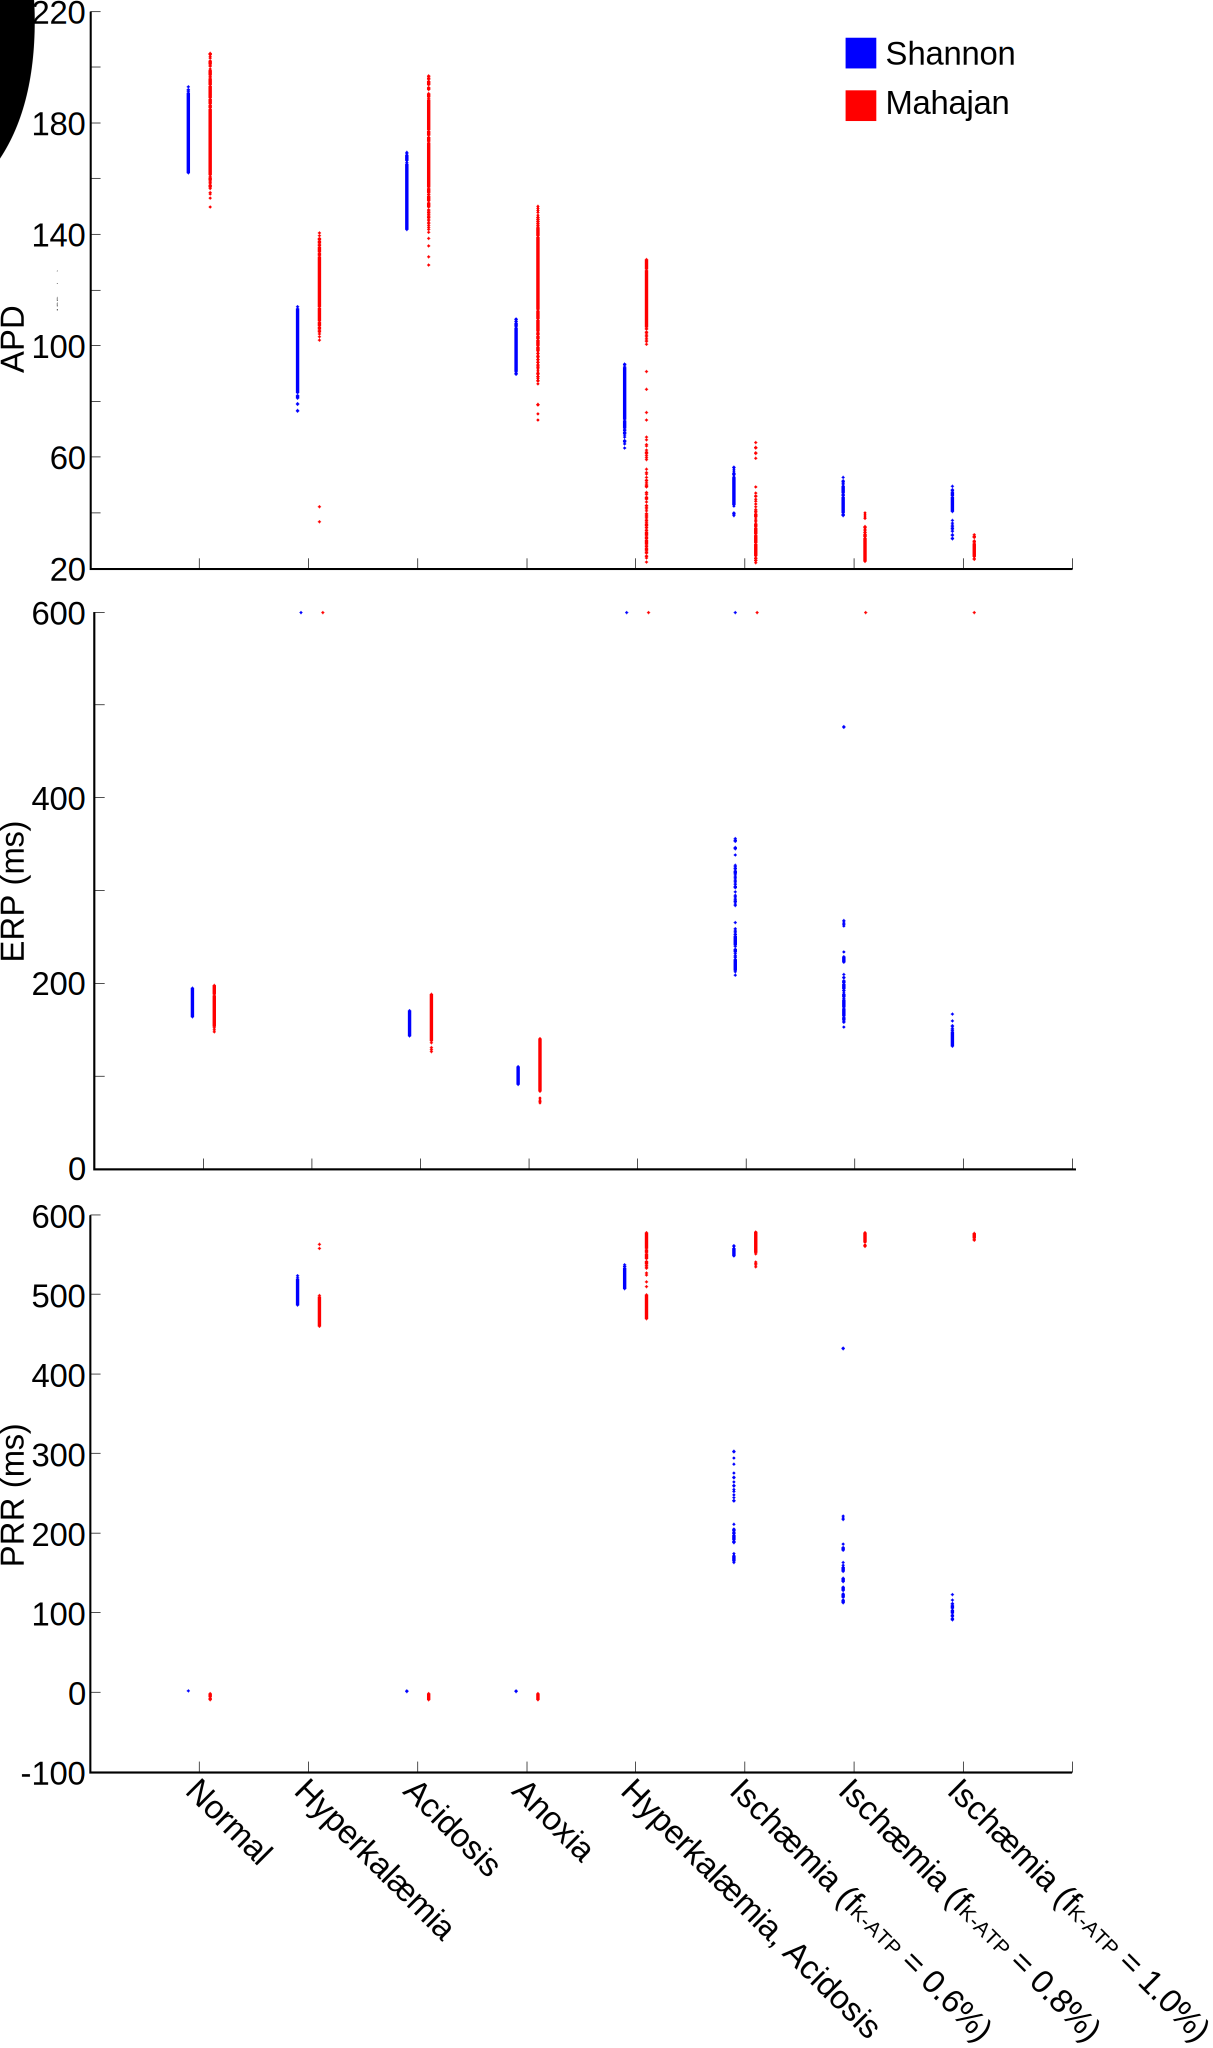
\includegraphics[width=0.7\textwidth]{discretePopulation}
 \caption[Distribution of biomarker values under specified conditions.]{Distribution of values within the population for non-failing models for APD\sub{90}, ERP and PRR, under specified conditions: normal (\ko = $5.4$ mM, \finhib{} = $0\%$, \fkatp{} = $0.0\%$, \fna{} = $0\%$), hyperkal\ae{}mia (\ko = $17.0$ mM, \finhib{} = $0\%$, \fkatp{} = $0.0\%$, \fna{} = $0\%$), acidosis (\ko = $5.4$ mM, \finhib{} = $25\%$, \fkatp{} = $0.0\%$, \fna{} = $0\%$), anoxia (\ko = $5.4$ mM, \finhib{} = $0\%$, \fkatp{} = $0.8\%$, \fna{} = $0\%$), hyperkal\ae{}mia and acidosis (\ko = $17$ mM, \finhib{} = $25\%$, \fkatp{} = $0.0\%$, \fna{} = $0\%$), and isch\ae{}mia with varying degrees of \fkatp{} activation (\ko = $5.4$ mM, \finhib{} = $0\%$, \fkatp{} = $\{0.6\%, 0.8\%, 1.0\%\}$, \fna{} = $0\%$).}
 \label{fig:discretePopulation}
\end{figure}

The Shannon population variation never exceeds the variation evident under `normal' conditions. The population distribution remains approximately normal at all stages during isch\ae{}mia, and the greatest rate of APD\sub{90} decline occurs in the first two minutes of isch\ae{}mia (according to mean response, and the decline of the population minimum and maximum values).

The Mahajan population also shows an initial decrease in variation, until 4 min PO, although the extent of the decrease in variation is not as great as with the Shannon population. Interestingly, both the maximum and minimum values of the population show a greater extent of decrease than the mean value during the first two minutes of isch\ae{}mia---this can be seen in the Mahajan histograms in Fig.~\ref{fig:isch-ap-apd90}, where the peak of the histogram moves from the left of the population at 0 min PO, to the right of the population at 2 min PO. After 4 min PO, however, the variation of the Mahajan population increases again, peaking at 8 min PO.

It is this peak in APD\sub{90} variation at 8 min PO that is of key importance for many of the effects seen within the Mahajan population under severe isch\ae{}mic conditions. This peak in variation occurs due to the population showing a continuum of dome collapse: some models show no evidence of dome collapse, while some other models seem to have almost complete dome collapse, with a range of models in between.  This range of models exhibits a behaviour that has a significant impact on the morphology of the AP, with a resultant impact on biomarkers such as APD\sub{90}. It should be noted that this `continuum' property of the Mahajan population is evident at several points in its analysis, and will be discussed further in \S\ref{sec:isch-modelFailure}. After this dome collapse continuum at 8 min PO, further isch\ae{}mic severity causes all models within the population to exhibit dome collapse---this is evident in Fig.~\ref{fig:isch-ap-apd90}

\begin{figure}
 \centering
 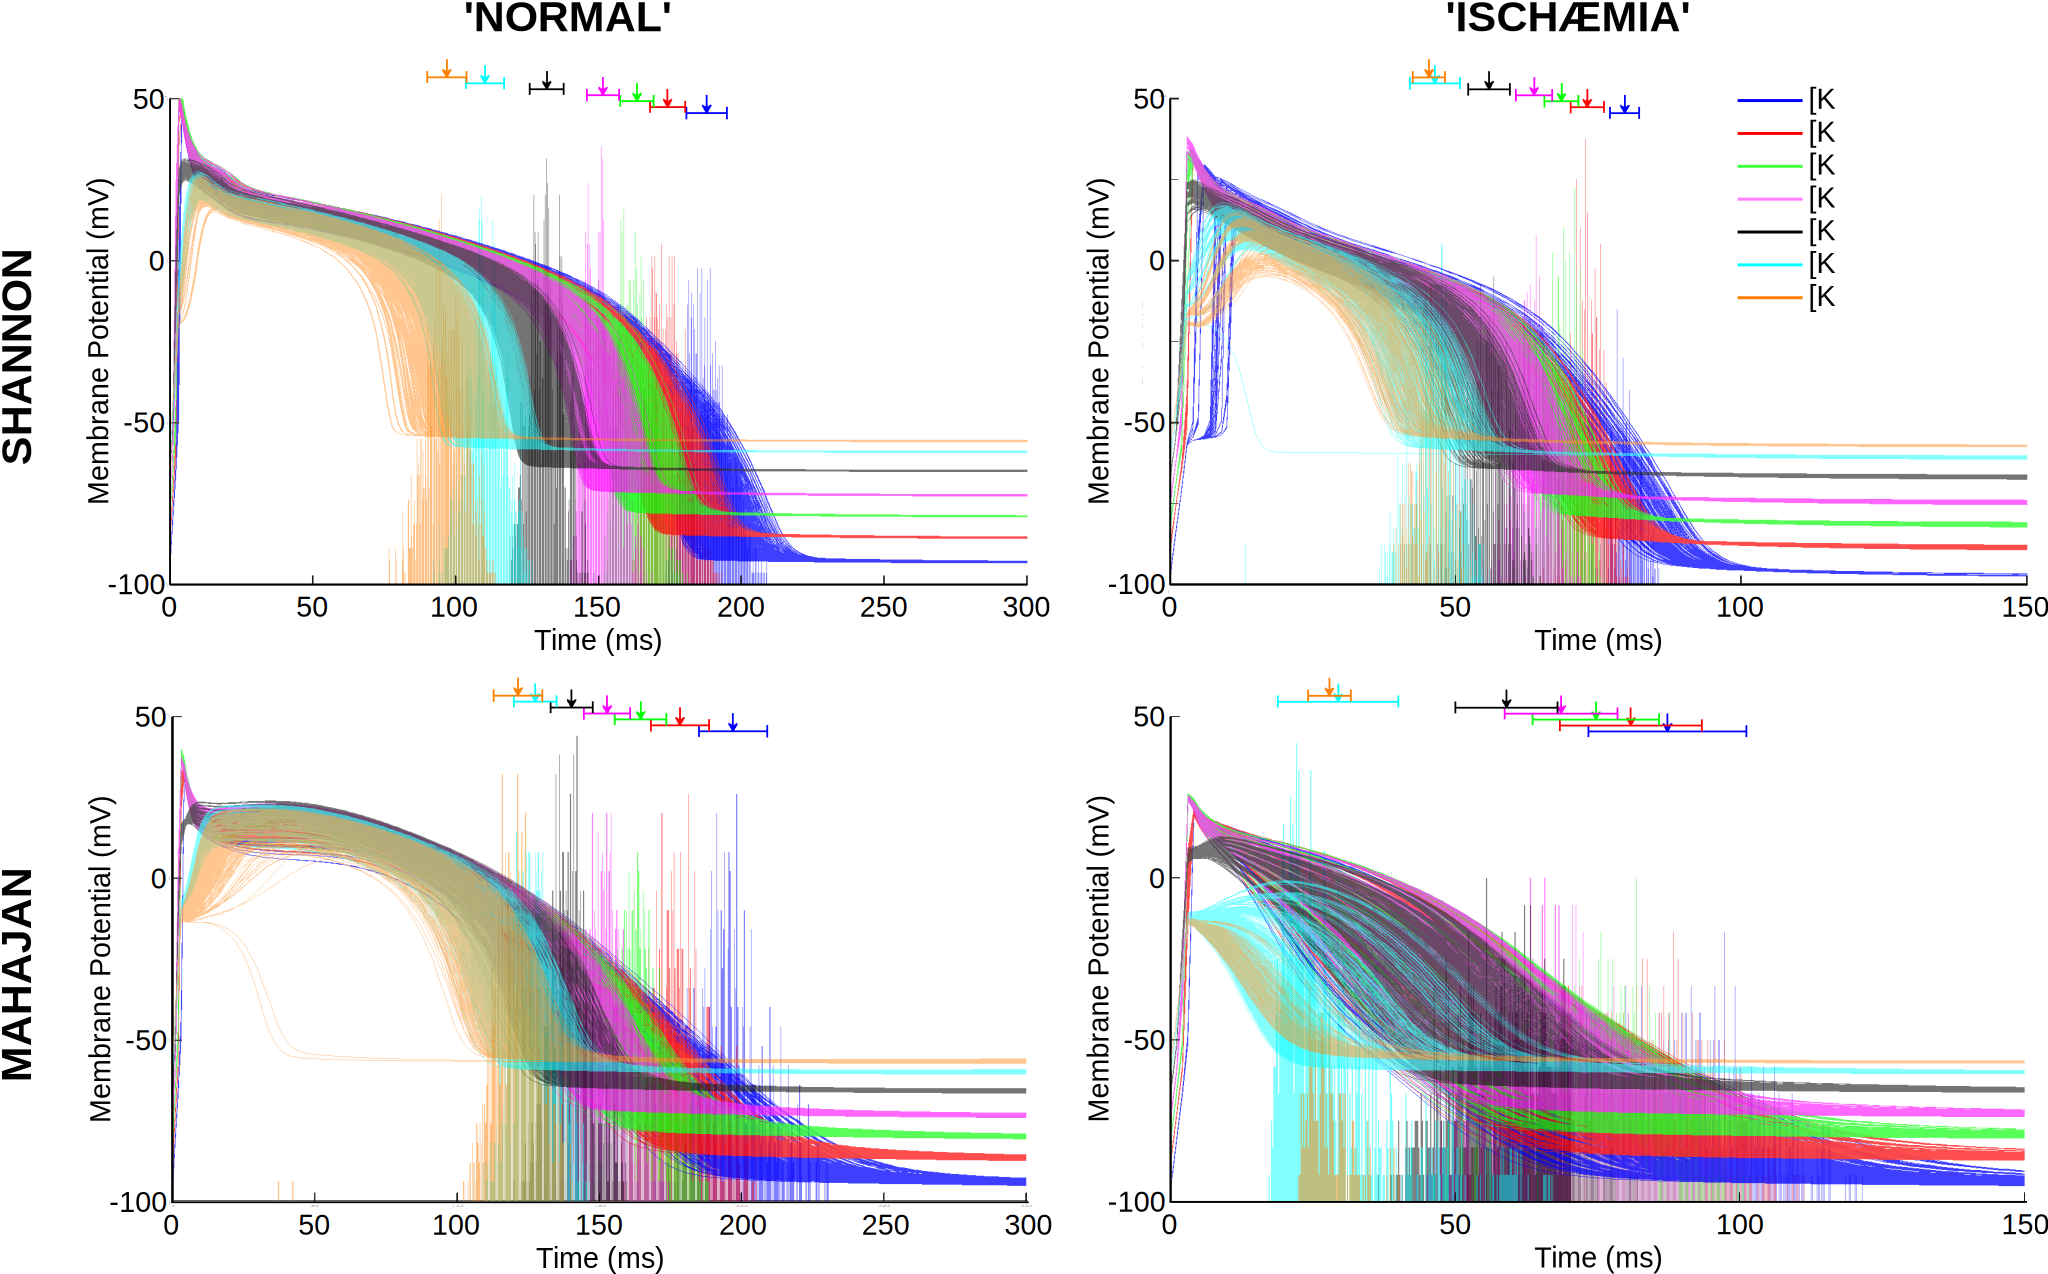
\includegraphics[width=0.8\textwidth]{ko_isch17-ap-full}
 \caption[Effect of \ko{} variation on the Shannon and Mahajan model populations.]{Effect of \ko{} variation on the Shannon and Mahajan (bottom) model populations. The histograms respresent the APD\sub{90} values associated with the populations.}
 \label{fig:ko_isch17-ap}
\end{figure}
% Weird shit going on with Ko going 15-17mM for both Shannon and Mahajan (minimum at 15)

\begin{figure}
 \centering
 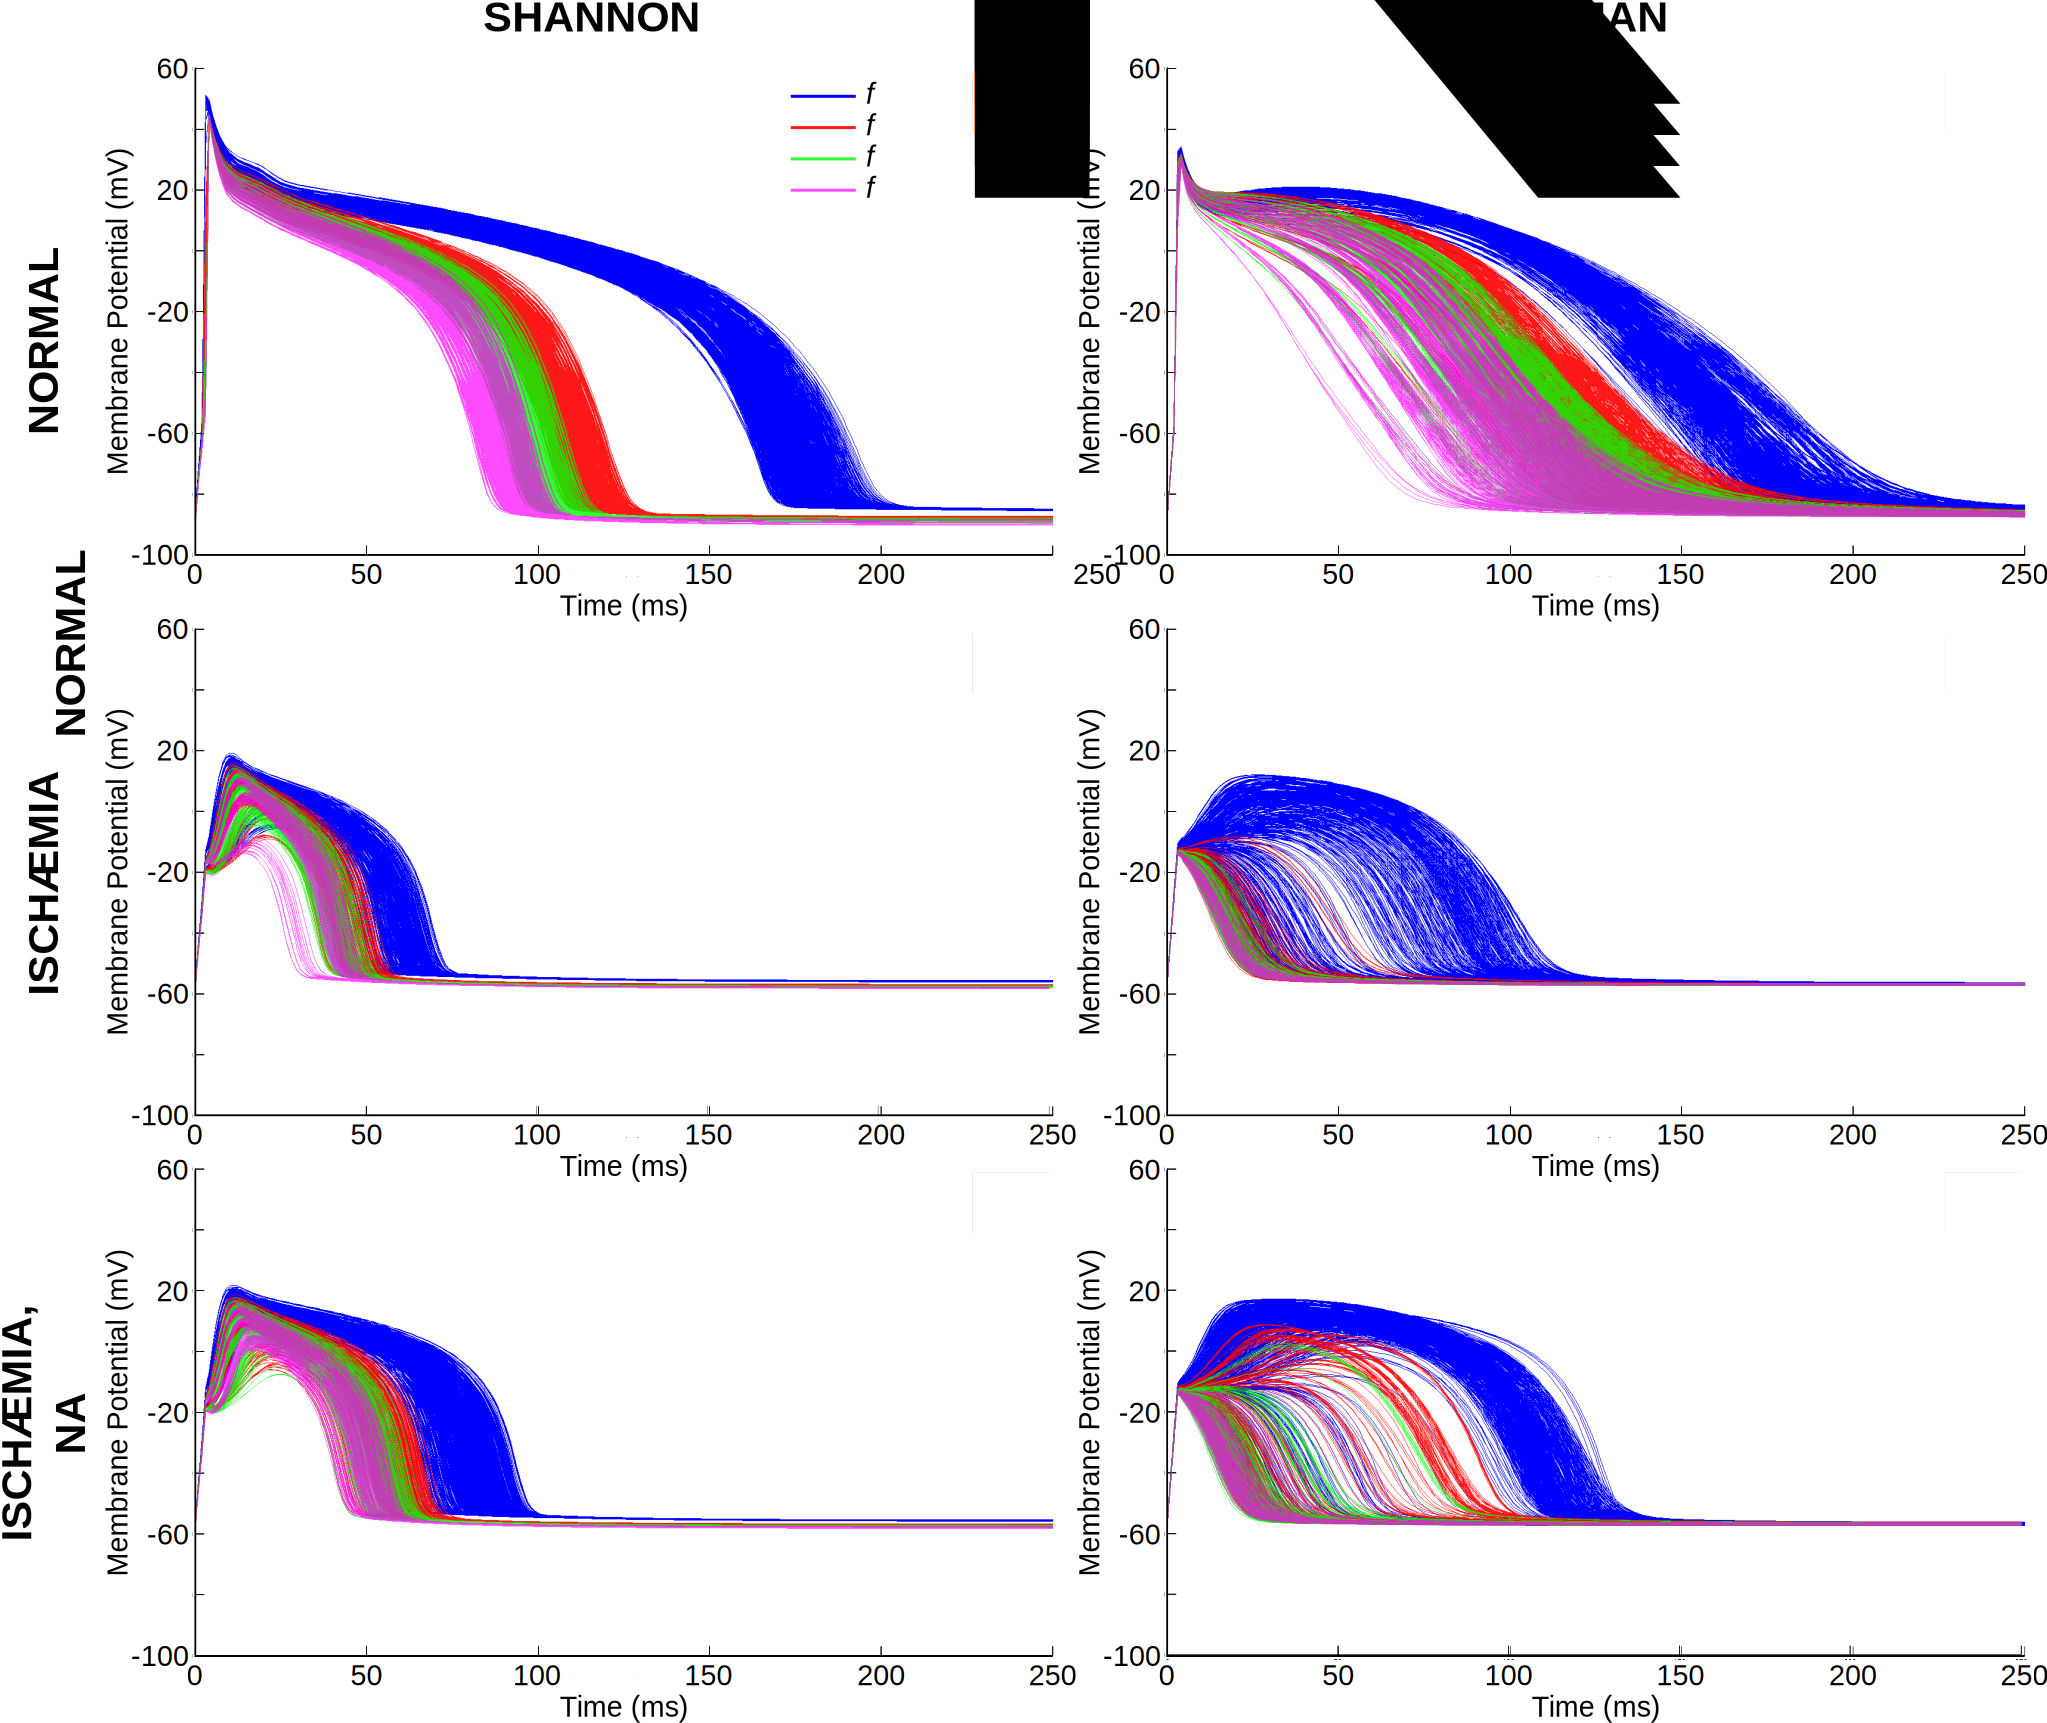
\includegraphics[width=\textwidth]{fkatp-ap}
 \caption[Effect of \fkatp{} variation on Shannon and Mahajan model populations.]{Effect of \fkatp{} variation on Shannon (left) and Mahajan (right) model populations given normal conditions (top, \ko = $5.4$ mM, \finhib{} = $0\%$, \fna{} = $0\%$), isch\ae{}mic conditions (middle, \ko = $17.0$ mM, \finhib{} = $25\%$, \fna{} = $30\%$), and isch\ae{}mic conditions where changes in the \na{} system of the cell are not modelled (bottom, \ko = $17.0$ mM, \finhib{} = $25\%$, \fna{} = $0\%$).}
 \label{fig:fkatp-ap}
\end{figure}
% Ischæmia without Na shown here to demonstrate how the 'normal' manner of investigating ischæmia can have different results to a more comprehensive simulation method
% Without Na change, slow repolarisation (min values comparable at all activations of IK-ATP) for Shannon. Similar effect for Mahajan, but that might be just a model failure situation rather than anything meaningful

% Mahajan not *completely* failing - still some vairation in min APD90 value, implying at least some action to attempt APD

% Mention importance of looking at overall population response, e.g. overall population spread via std or inspection of histograms. Massive increase in range many not be important...

% Isch K+ effect -> spatial variation

\subsection{ERP and PRR}
\label{subsec:isch-erpprr-response}
% Caution regarding calculation of ERP, and thus of calculating PRR

\begin{table}
 \centering
 \begin{tabular}{cccc|r@{ }lr@{ }l|r@{ }lr@{ }l}
  \ko{}	& \multirow{2}{*}{\fkatp{}}	& \multirow{2}{*}{\finhib{}}	& \multirow{2}{*}{\fna{}}	& \multicolumn{4}{c|}{Shannon}	& \multicolumn{4}{c}{Mahajan}	\\
  (mM)	&	&	&	& \multicolumn{2}{c}{Failure}	& \multicolumn{2}{c|}{ERP$\ge$CL}	& \multicolumn{2}{c}{Failure}	& \multicolumn{2}{c}{ERP$\ge$CL}	\\
  \hline
  \hline
  $5.4$		& $0.00$	& $0$	& $0$	& \multicolumn{2}{c}{$0$}	& \multicolumn{2}{c|}{$0$}	& \multicolumn{2}{c}{$0$}	& \multicolumn{2}{c}{$0$}	\\
  $7.72$	& $0.16$	& $5$	& $6$	& \multicolumn{2}{c}{$0$}	& \multicolumn{2}{c|}{$0$}	& \multicolumn{2}{c}{$0$}	& \multicolumn{2}{c}{$0$}	\\
  $10.04$	& $0.32$	& $10$	& $12$	& \multicolumn{2}{c}{$0$}	& \multicolumn{2}{c|}{$0$}	& \multicolumn{2}{c}{$0$}	& \multicolumn{2}{c}{$0$}	\\
  $12.36$	& $0.48$	& $15$	& $18$	& \multicolumn{2}{c}{$0$}	& \multicolumn{2}{c|}{$0$}	& \multicolumn{2}{c}{$0$}	& \multicolumn{2}{c}{$0$}	\\
  $14.68$	& $0.64$	& $20$	& $24$	& \multicolumn{2}{c}{$0$}	& \multicolumn{2}{c|}{$0$}	& \multicolumn{2}{c}{$0$}	& \multicolumn{2}{c}{$0$}	\\
  $17.0$	& $0.80$	& $25$	& $30$	& $605$		& $(44.7\%)$	& \multicolumn{2}{c|}{$0$}	& $613$		& $(78.7\%)$	& $166$		& $(100\%$)	\\
  \hline
  $17.0$	& $0.60$	& $25$	& $30$	& $414$		& $(30.6\%)$	& $471$		& $(50.2\%)$	& $578$		& $(78.7\%)$	& $201$		& $(100\%$)	\\
  $17.0$	& $1.00$	& $25$	& $30$	& $847$		& $(62.6\%)$	& \multicolumn{2}{c|}{$0$}	& $720$		& $(78.7\%)$	& $59$		& $(100\%$)	\\
  \hline
  $17.0$	& $0.00$	& $0$	& $0$	& $3$		& $(0.0\%)$	& $1349$	& $(100\%)$	& \multicolumn{2}{c}{$0$}	& $779$		& $(100\%)$	\\
  $5.4$		& $0.80$	& $0$	& $0$	& \multicolumn{2}{c}{$0$}	& \multicolumn{2}{c|}{$0$}	& \multicolumn{2}{c}{$0$}	& \multicolumn{2}{c}{$0$}	\\
  $5.4$		& $0.00$	& $25$	& $0$	& \multicolumn{2}{c}{$0$}	& \multicolumn{2}{c|}{$0$}	& \multicolumn{2}{c}{$0$}	& \multicolumn{2}{c}{$0$}	\\
  $5.4$		& $0.00$	& $0$	& $30$	& \multicolumn{2}{c}{$0$}	& \multicolumn{2}{c|}{$0$}	& \multicolumn{2}{c}{$0$}	& \multicolumn{2}{c}{$0$}	\\
  \hline
  $5.4$		& $0.80$	& $25$	& $30$	& \multicolumn{2}{c}{$0$}	& $1349$	& $(100\%)$	& \multicolumn{2}{c}{$0$}	& $779$		& $(100\%)$	\\
  $17.0$	& $0.00$	& $25$	& $30$	& $72$		& $(5.3\%)$	& $1280$	& $(100\%)$	& $183$		& $(23.5\%)$	& $596$		& $(100\%)$	\\
  $17.0$	& $0.80$	& $0$	& $30$	& $150$		& $(11.1\%)$	& $192$		& $(16.0\%)$	& $432$		& $(55.5\%)$	& $347$		& $(100\%)$	\\
  $17.0$	& $0.80$	& $25$	& $0$	& $411$		& $(30.4\%)$	& $82$		& $(8.7\%)$	& $584$		& $(75.0\%)$	& $193$		& $(99.0\%)$	\\
 \end{tabular}
 \caption[Model failure \& ERP prolongation.]{Effect of different conditions associated with isch\ae{}mia on the number of models within the populations that fail, and of those that do not fail, those which exhibit ERP$\ge$CL. The first group represent those conditions simulating linear progression from normal to isch\ae{}mic conditions; the second group represent isch\ae{}mic conditions with decreased/increased \ikatp{} activation; the third group represent each individual change in isch\ae{}mia applied individually; the fourth group represent isch\ae{}mia when one condition remains `normal'.}
 \label{table:isch-fail_erp}
\end{table}

\begin{figure}
 \centering
 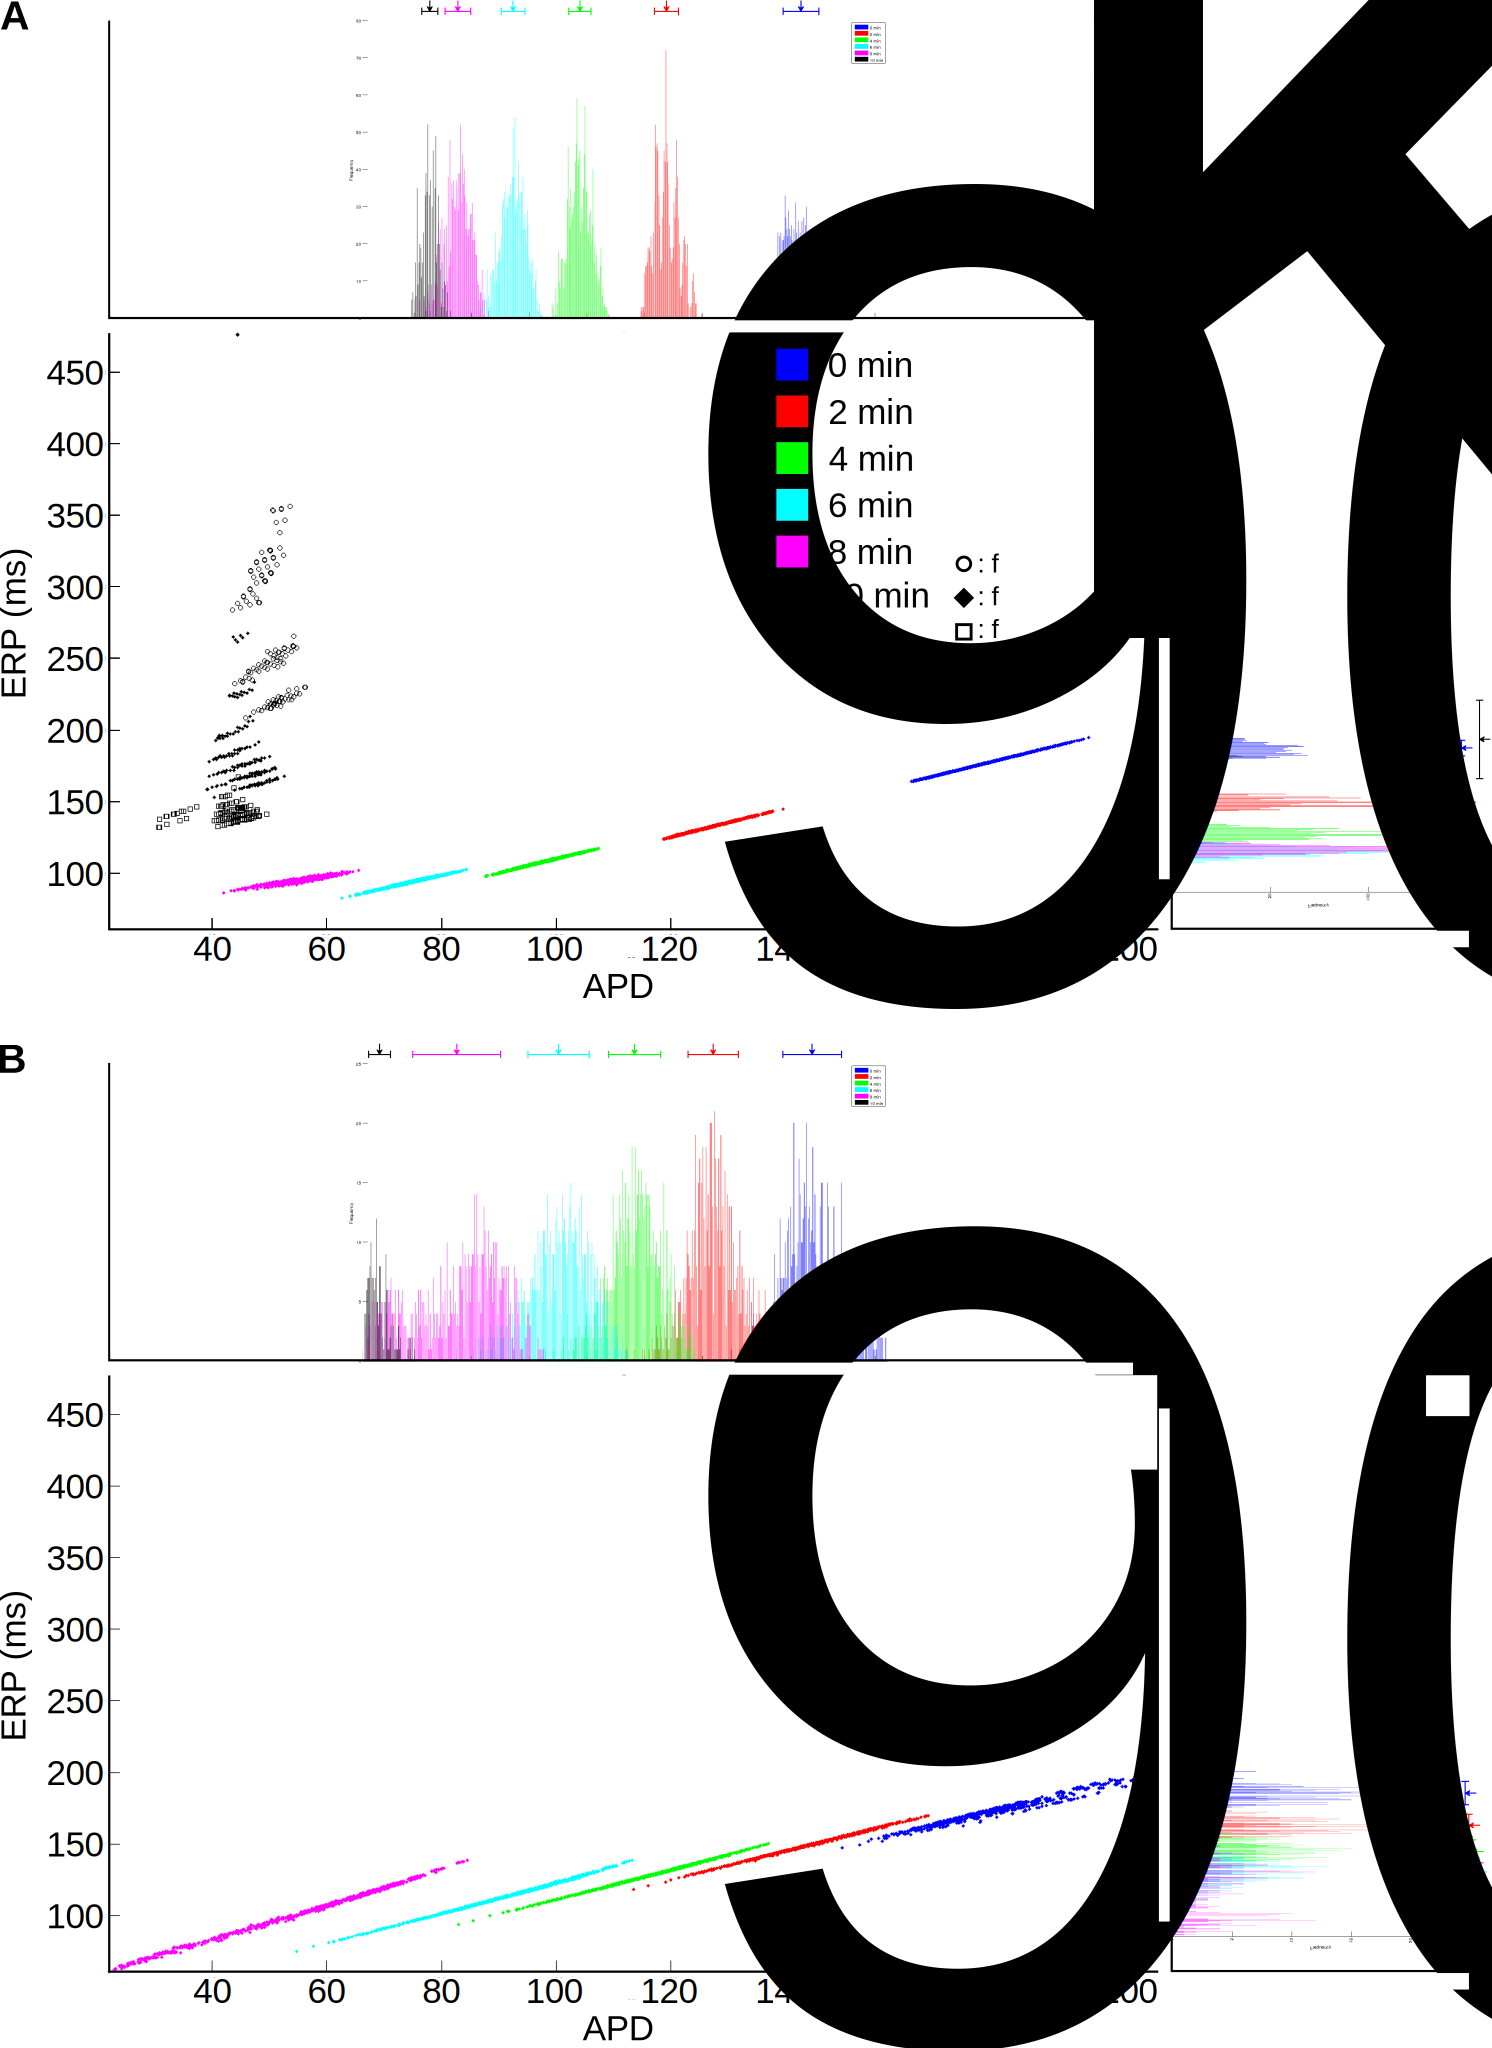
\includegraphics[width=0.8\textwidth]{isch17-apd90_erp-fkatpVar}
 \caption[Relation between APD\sub{90} and ERP during isch\ae{}mia.]{Relation between APD\sub{90} and ERP at various points during isch\ae{}mia for the Shannon (A) and Mahajan (B) populations. For 10 min PO, the APD\sub{90}/ERP relation is also shown for increased/decreased \fkatp{} at 10 min PO. Histograms using the same scales as the main plot are given: APD\sub{90} above the main plot, ERP to the right.}
 \label{fig:isch17-apd90_erp-fkatpVar}
\end{figure}

\begin{figure}
 \centering
 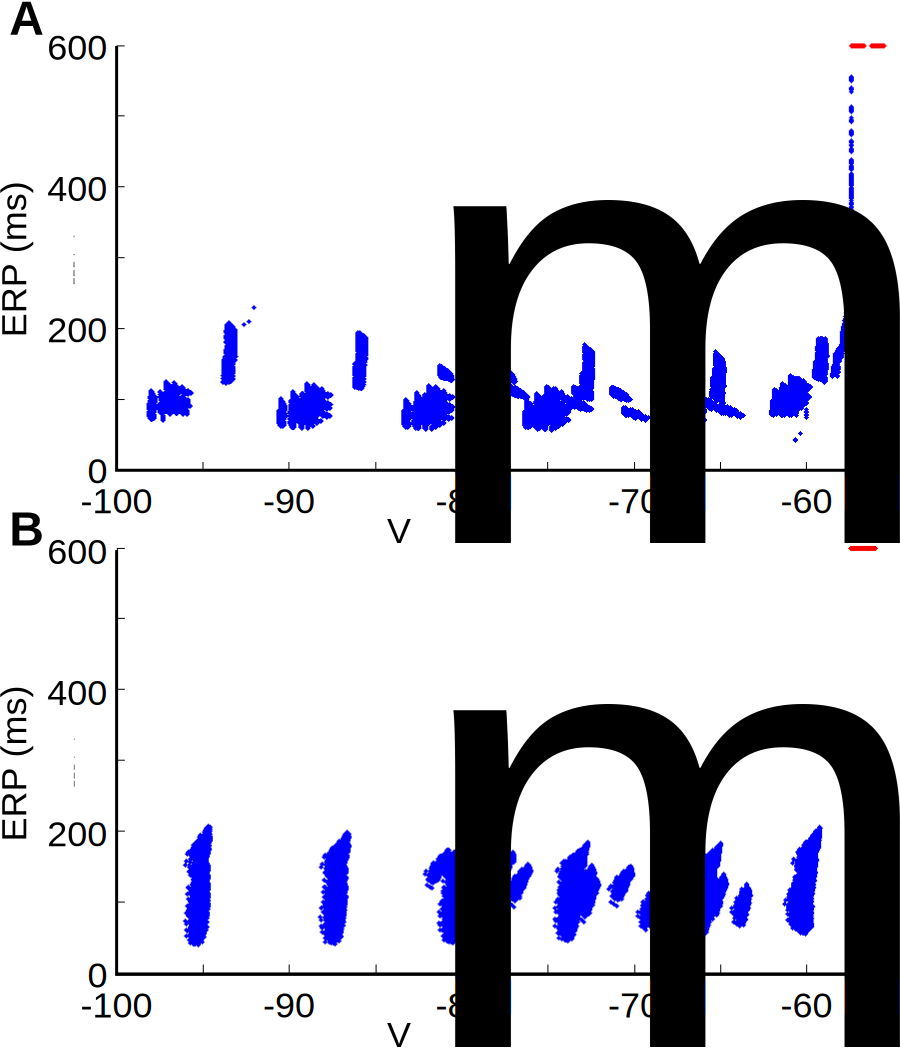
\includegraphics[width=0.8\textwidth]{population-vmin_erp}
 \caption[Relation between \vrest{} and ERP across both populations for all simulated conditions.]{Relation between \vrest{} and ERP across Shannon (A) and Mahajan (B) populations for all simulated conditions. Those models with ERP$\ge$CL are highlighted in red.}
 \label{fig:population-vmin_erp}
\end{figure}
% Mention overlap of relations (and the link to threshold values, though no relation with hj values)

% Limitations of ERP calculation for severe ischæmia (ERP > 600 ms)
% Very small variation in PRR => high correlation between APD90 and ERP, which declines with increasing ischæmic severity (though APD90/ERP mean, etc., can indicate PRR, not always accurate)
% APD90/ERP relation highly dependent on conditions

\subsection{Other Biomarkers}
\label{subsec:isch-other-response}
% Vmax: occurs later if during Phase 2, thus provides other source of excitation - arrhythmogenic?
% Link between Vrest and dVdt/ERP - both validation
%	Variation in Vrest not modelled well - implications here?

\section{Model Failure During Isch\ae{}mia}
\label{sec:isch-modelFailure}
% Critique method criterion used - why does Shannon have cut-off between failing/nonfailing, but not Mahajan? Where does this value come from?

\begin{figure}
 \centering
 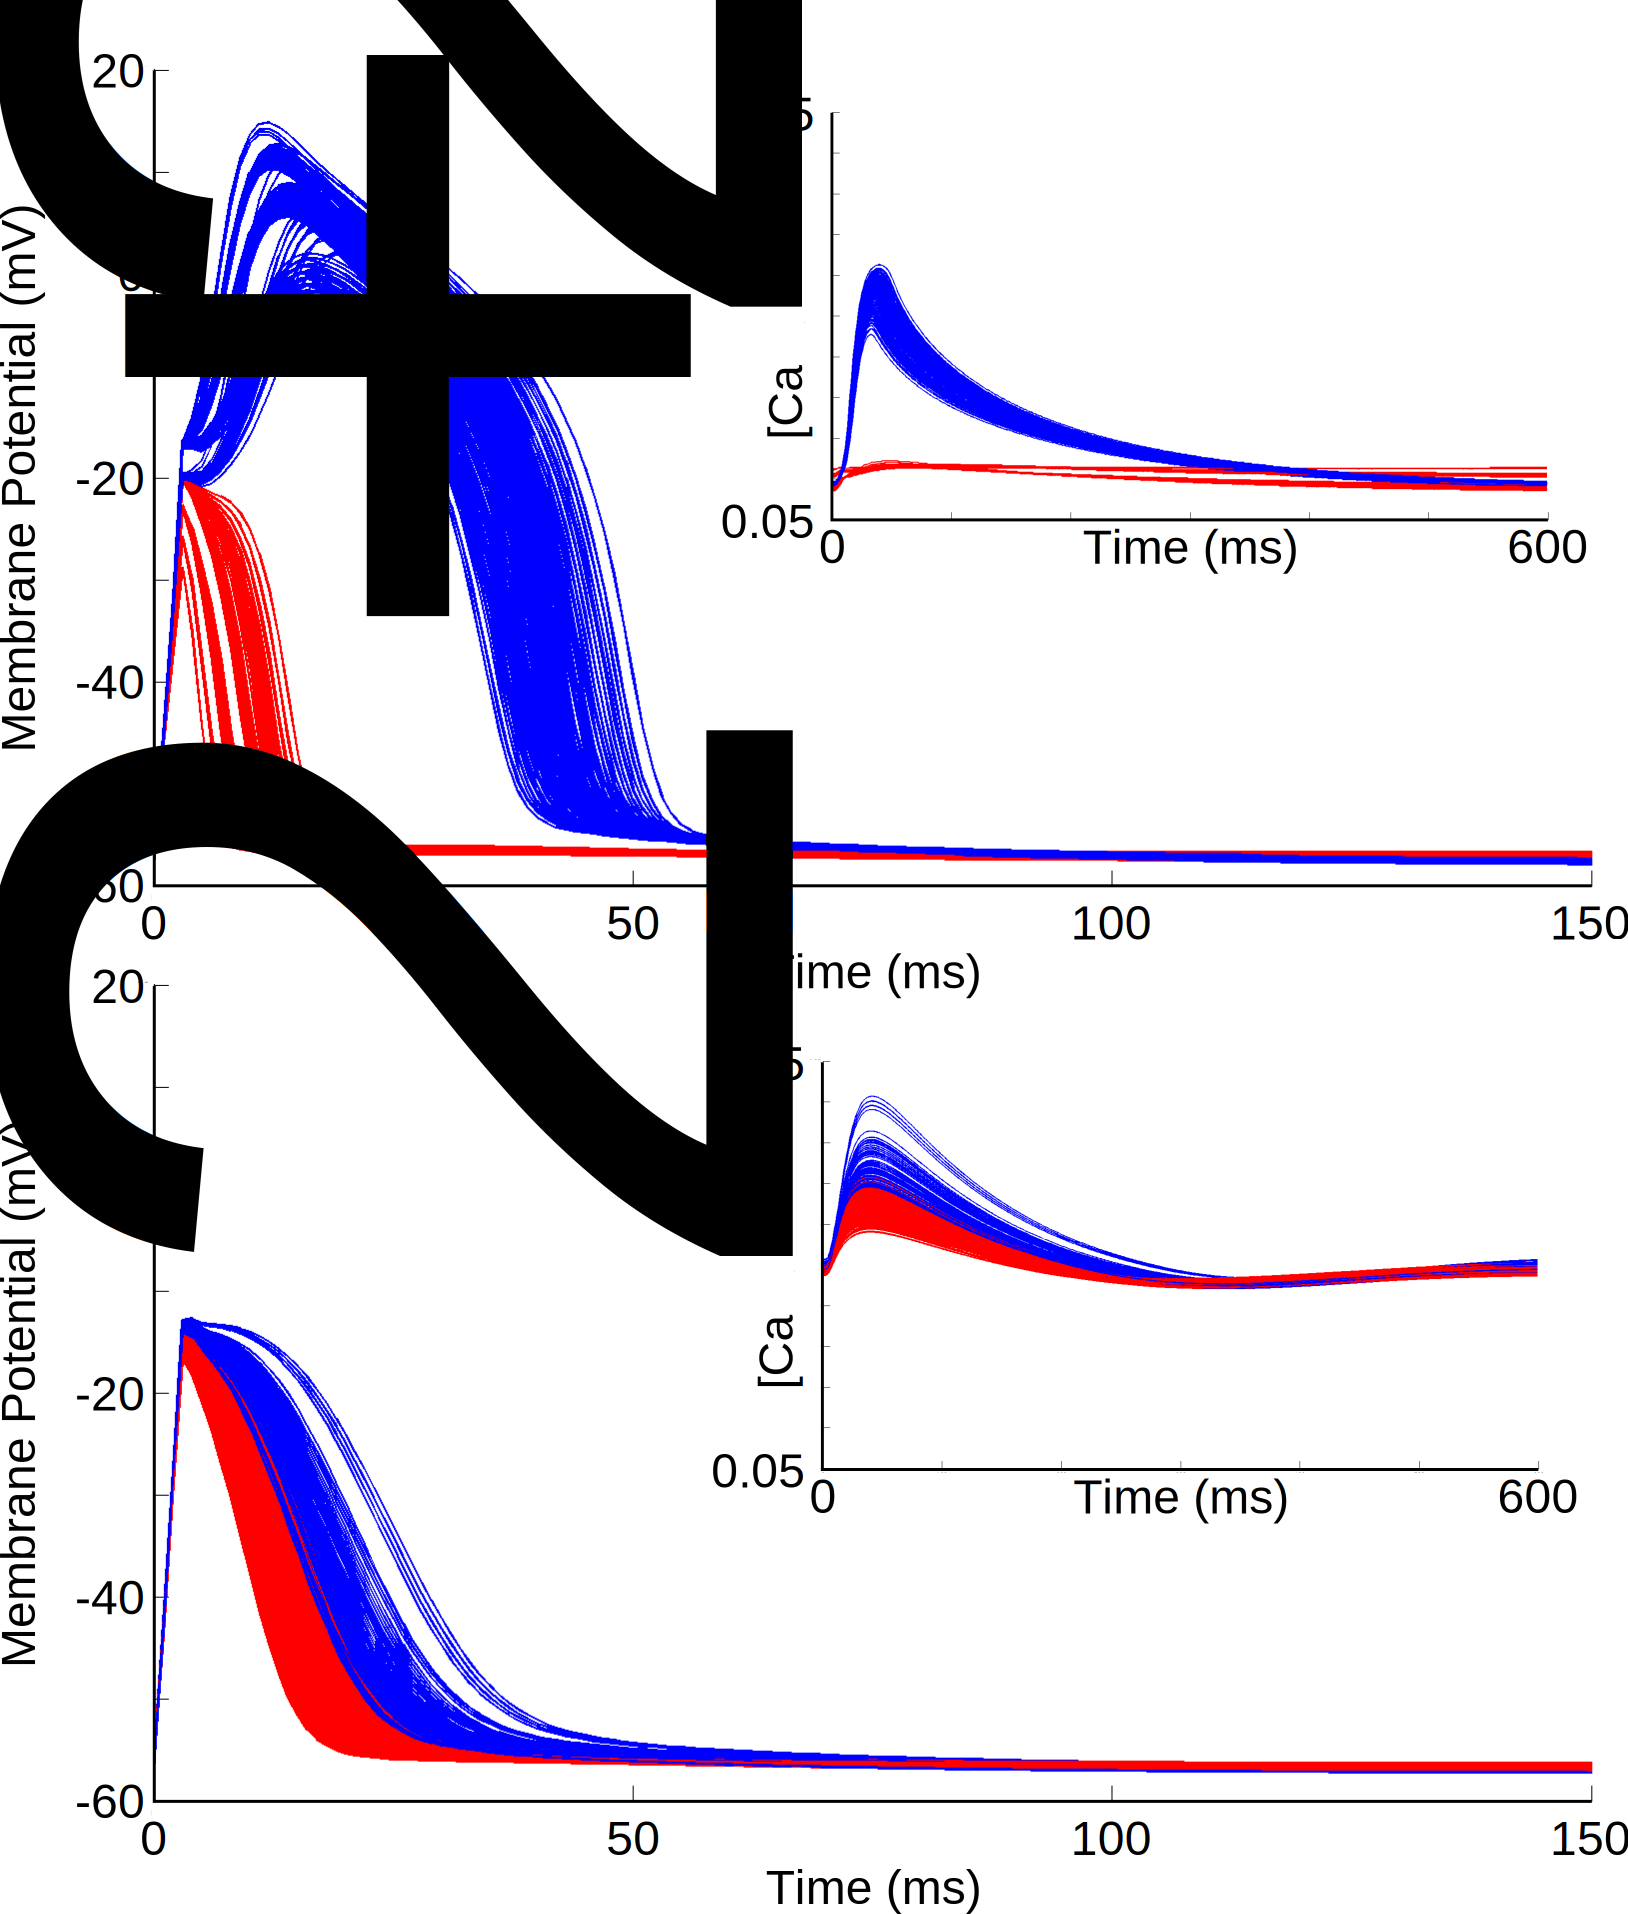
\includegraphics[width=0.8\textwidth]{fail-isch17}
 \caption[Illustration of failing and non-failing APs during isch\ae{}mia.]{Illustration of failing and non-failing APs at 10 min PO for the Shannon (A) and Mahajan (B) populations; APs classed as non-failing are shown in blue, those classed as failing are shown in red. \emph{Inset:} Data for \cai{}.}
 \label{fig:fail-isch17}
\end{figure}

\biblio

\end{document}